%!TEX root = ../final_report.tex

\textit{Include any formulas, pseudocode, diagrams -- anything that is necessary to clearly explain your system and what you have done. If possible, illustrate the intermediate stages of your approach with result images.}

For our approach, we implemented a variation on the CVPR 2015 paper from Eitel et al titled \textit{Multimodal Deep Learning for Robust RGB-D Object Recognition} \cite{Eitel2015}. The main contribution of this paper was to show how pretrained networks such as AlexNet or VGGNet can be used to process single-channel depth information, enabling networks to run on depth information despite a lack of large-scale depth datasets such as ImageNet for color images \cite{ImageNet2015}. In this section, we will discuss our network architecture, our preprocessing phase, and our training methodology.

\subsection{Dataset}
In this project, we use Washington RGB-D object dataset \cite{Lai2011_rgbddata} . This dataset includes 300 common household object, divided into 51 categories (Figure \ref{fig:rgbd_dataset}). Using a Kinect style 3D camera, data are recorded, synchronized, and aligned at the framerate of 30Hz and resolution of 640 x 480. Each object is recorded while being placed on a turntable under three different camera viewpoints: low, middle, and high. 

\begin{figure}[htbp]
	\centering
	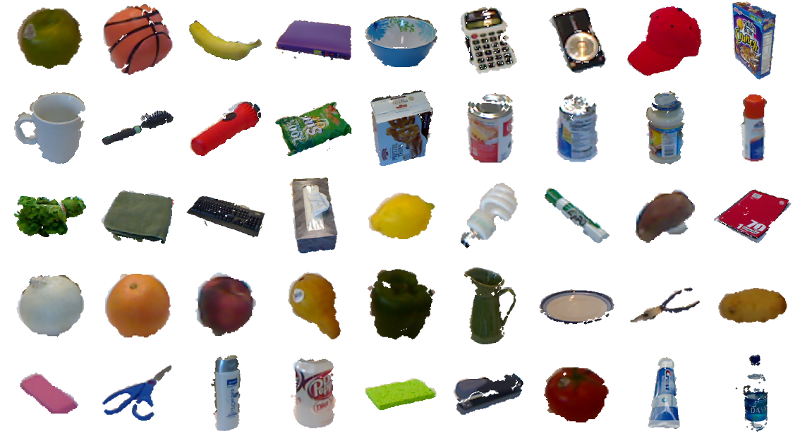
\includegraphics[width=0.85\linewidth]{img/rgbd_dataset2.png}
	\caption{Some samples from RGB-D Object Dataset.}
	\label{fig:rgbd_dataset}
\end{figure}

The dataset is structured as follow:
\begin{verbatim}
    <category>/<object_id>/<sample_id>
\end{verbatim}
where
\begin{verbatim}
    <object_id> = <category>_<number>
\end{verbatim}
and
\begin{verbatim}
    <sample_id> = <category>_<number>_<video>_<frame>
\end{verbatim}
For example
\begin{verbatim}
    banana/banana_1/banana_1_2_5
\end{verbatim}
means that the sample is the fifth frame of the second video sequence (out of three different camera viewpoints). This sample records object \texttt{banana\_1}, which is the first object in \texttt{banana} category. Each video sequence contains around 150 samples.

For each sample, there are four different kinds of data: color image (Figure \ref{fig:orig_img}a), depth image (Figure \ref{fig:orig_img}b), segmentation mask (Figure \ref{fig:img_mask}), and a text file indicating the top-left corner of the object of interest.

\begin{figure}[htbp]
	\centering
	\begin{subfigure}[b]{0.45\linewidth}
		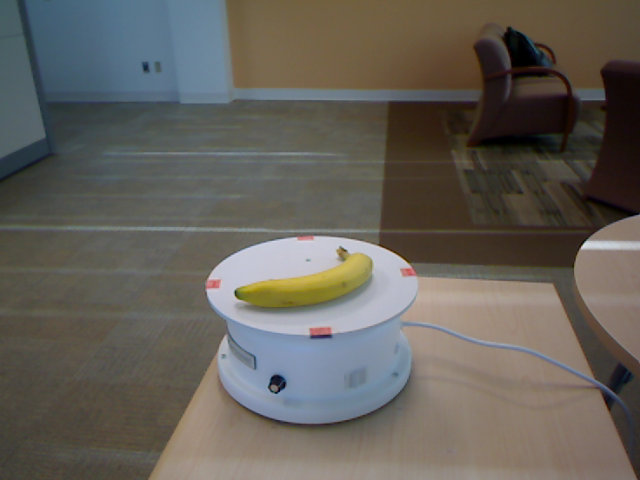
\includegraphics[width=\textwidth]{img/banana_1_1_1.png}
		\caption{Color image}
	\end{subfigure}   	
	\begin{subfigure}[b]{0.45\linewidth}
		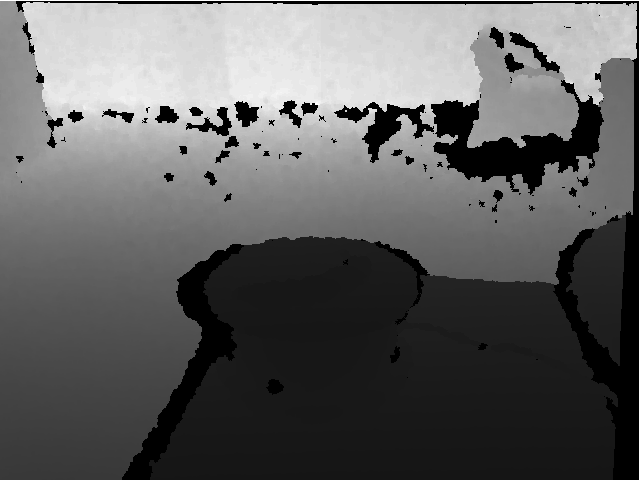
\includegraphics[width=\textwidth]{img/banana_1_1_1_depth.png}
		\caption{Depth image}
	\end{subfigure}
	\caption{Original color and depth photos of object captured on a turntable.}
	\label{fig:orig_img}
\end{figure}

\begin{figure}[htbp]
	\centering
	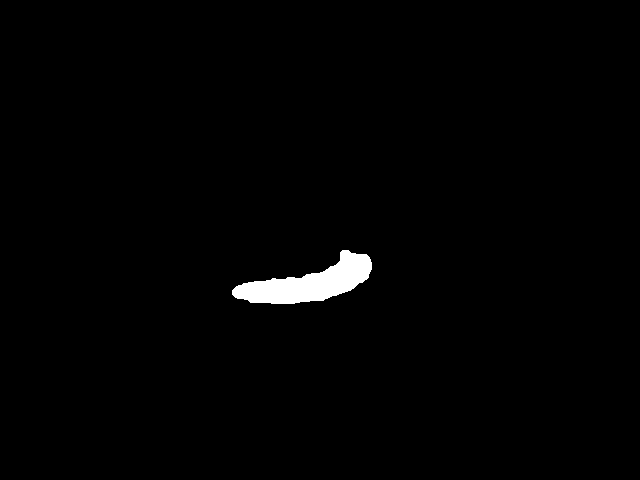
\includegraphics[width=0.5\linewidth]{img/banana_1_1_1_mask.png}
	\caption{Ground-truth segmentation mask for banana object.}
	\label{fig:img_mask}
\end{figure}

\subsection{Network Architecture}
The network structure proposed by Eitel et al \cite{Eitel2015} is pictured in Figure \ref{fig:network}. Its structure can be broken into three parts: a network for color-based classification, a network for depth-based classification, and a final fusion network combining the two single-modality streams into a final classification result. Fusing two single-stream networks is beneficial for two main reasons. Firstly, unlike large companies like Microsoft and Google who have recently become involved in deep learning competitions, we do not have a GPU farm at our disposal to train networks ad-infinitum. Additionally, the first consumer depth camera was only released within the last 5 years \cite{Alex2009_kinect}. Unlike ImageNet, we do not have millions of labeled depth captures to use for network training. A smaller dataset could be used to train a depth network from scratch, but using such a comparatively small dataset would likely result in network overfitting and poor results on test data.

\begin{figure}[htbp]
	\centering
	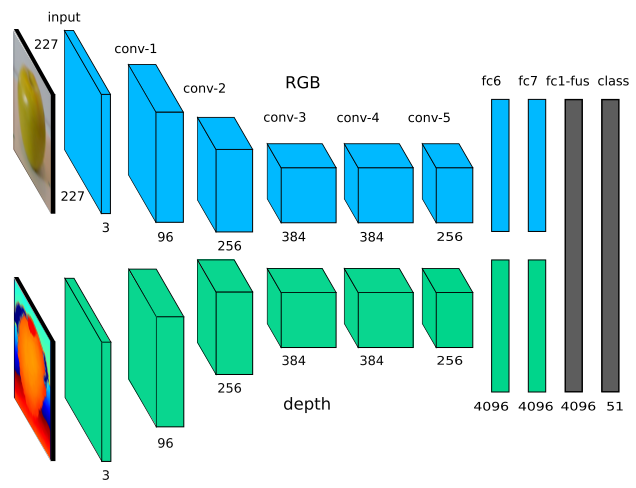
\includegraphics[width=0.85\linewidth]{img/architecture.png} 
	\caption{Network architecture using separate color and depth inputs. Inputs for color and depth are $227 \times 227 \times 3$, assuming depth colorization during preprocessing stage. Each modality has its own individual network, with the two resultant fusion layers providing final classification.}
	\label{fig:network}
\end{figure}

To this end, we use the pretrained network AlexNet for our single stream network. AlexNet is a top-tier network without as many layers as a deep residual learning network, making it a better choice for our limited compute capacity and timeframe. Our implementation of AlexNet is shown in further detail in Figure \ref{fig:single_stream_layout}. 

Finally, we strip the \texttt{fc8} classification layers from the our AlexNet streams and concatenate the two models, feeding the now 8092-node layer into \texttt{fc1-fus}, a 4096-node fully-connected layer. This then goes into a final classification layer with softmax activation. The individual elements of the network are described below.

\begin{figure}[htbp]
	\begin{mdframed}
		\begin{itemize}
			\item \texttt{conv-1}:
			\begin{itemize}
				\item $96 \times 11 \times 11$ Convolutional Filter
				\item ReLU Activation
				\item Batch Normalization
				\item $2 \times 2$ Max Pooling
			\end{itemize}
			\item \texttt{conv-2}:
			\begin{itemize}
				\item 2-width Zero Padding
				\item $256 \times 5 \times 5$ Convolutional Filter
				\item ReLU Activation
				\item Batch Normalization
				\item $2 \times 2$ Max Pooling
			\end{itemize}
			\item \texttt{conv-3}:
			\begin{itemize}
				\item 1-width Zero Padding
				\item $384 \times 3 \times 3$ Convolutional Filter
				\item ReLU Activation
			\end{itemize}
			\item \texttt{conv-4}:
			\begin{itemize}
				\item 1-width Zero Padding
				\item $384 \times 3 \times 3$ Convolutional Filter
				\item ReLU Activation
			\end{itemize}
			\item \texttt{conv-5}:
			\begin{itemize}
				\item 1-width Zero Padding
				\item $256 \times 3 \times 3$ Convolutional Filter
				\item ReLU Activation
				\item $2 \times 2$ Max Pooling
			\end{itemize}
			\item \texttt{fc6}:
			\begin{itemize}
				\item 4096-node Fully Connected Layer
				\item ReLU Activation
				\item 50\% Dropout
			\end{itemize}
			\item \texttt{fc7}:
			\begin{itemize}
				\item 4096-node Fully Connected Layer
				\item ReLU Activation
				\item 50\% Dropout
			\end{itemize}
			\item \texttt{fc8}:
			\begin{itemize}
				\item 51-node Fully Connected Layer
				\item Softmax Activation
			\end{itemize}
		\end{itemize}
	\end{mdframed}
	\caption{Single-stream network layout for depth and color channels respectively. Dropout layers are removed during test time.}
	\label{fig:single_stream_layout}
\end{figure}

\subsubsection{Convolutional Layer}
TODO, what is a convolutional layer

\subsubsection{ReLU}
TODO, what is ReLU

\subsubsection{Batch Normalization}
TODO, what is Batch Normalization

\subsubsection{Max Pooling}
TODO, what is max pooling




\subsection{Preprocessing}

Preprocessing for this network has three primary stages: segmentation, rescaling, and depth colorization. First, we segment the color and depth images using a mask provided with the dataset, setting pixel values to black in the color image and zero in the depth image (Figure \ref{fig:img_cropped}). Our dataset provides segmentation masks for every object capture in the dataset, although Eitel et al \cite{Eitel2015} showed in their paper that doing classification without the segmentation mask was also possible.

\begin{figure}[htbp]
	\centering
	\begin{subfigure}[b]{0.45\linewidth}
		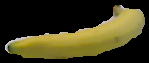
\includegraphics[width=\textwidth]{img/banana_1_1_1_crop.png}
		\caption{Color image}
	\end{subfigure}   	
	\begin{subfigure}[b]{0.45\linewidth}
		
\includegraphics[width=\textwidth]{img/banana_1_1_1_depth_crop.png}
		\caption{Depth image}
	\end{subfigure}
	\caption{Cropped banana photo using given segmentation mask.}
	\label{fig:img_cropped}
\end{figure}

The image pairs are then cropped and rescaled to $227 \times 227$, the size of the input for the single-stream networks. We do this by scaling the image by a factor:

\[ \kappa = \frac{\max(W, H)}{227}. \]

where $W$ and $H$ are object's width and height, respectively. The smaller dimension is then zero-padded to fit the square $227 \times 227$. By this way the object is kept as the image's center, making it efficient in case the boundary is cropped during training (Figure \ref{fig:depth_colorized}a). More interesting, however, is the process of depth colorization ((Figure \ref{fig:depth_colorized}b)). Depth sensors like the Xbox Kinect only give a single-channel intensity image proportional to the distance from the sensor. By converting depth images into three-channel data, we can treat them as images and feed into AlexNet (or other pretrained image recognition networks). Although there are different ways to colorize depth maps, jet colorization is proven superior in term of boosting system's performance \cite{Eitel2015}.

\begin{figure}[htbp]
	\centering
	\begin{subfigure}[b]{0.45\linewidth}
		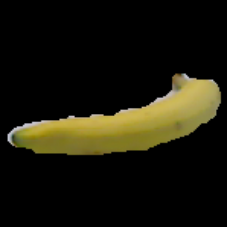
\includegraphics[width=\textwidth]{img/banana_1_1_1_resize.png}
		\caption{Color image}
	\end{subfigure}   	
	\begin{subfigure}[b]{0.45\linewidth}
		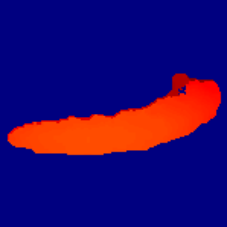
\includegraphics[width=\textwidth]{img/banana_1_1_1_depth_resize.png}
		\caption{Depth image}
	\end{subfigure}
	
	\caption{Rescaled cropped color photo and rescaled cropped depth photo colorized using \textit{Jet} heatmap.}
	\label{fig:depth_colorized}
\end{figure}





\subsection{Network Training}
The training process in divided into two different phases: (1) training the stream networks and (2) training the fusion network. Suppose that we have the dataset
\[ \mathcal{D} = \left\{ \left(\mathbf{x}^1, \mathbf{d}^1, \mathbf{y}^1\right), ..., \left(\mathbf{x}^N, \mathbf{d}^N, \mathbf{y}^N\right) \right\} \]
where $\mathbf{x}^i$ is a RGB image, $\mathbf{d}^i$ is a depth image, and $\mathbf{y}^i$ is a label in the form of
\[
\mathbf{y}^i = (y_1^i, y_2^i, ..., y_k^i, ..., y_{M}^i)^\top \qquad \text{s.t.} \qquad y_k^i = 
\begin{cases}
1, & \mathbf{x}^i \text{ and } \mathbf{d}^i \text{ belong to class } k\\
0, & \text{otherwise}
\end{cases}
\]
where $M$ is the number of classes. The data are fed into the first training phase and then the second one.

\subsubsection{Training the stream networks}
Let $g^I(\mathbf{x}^i; \theta^I)$ be the representation for the color image $\mathbf{x}^i$ of the last fully connected layer from stream networks (\textit{fc7}) of AlexNet, where $\theta^I$ is the parameter. Similarly, we have $g^D(\mathbf{d}^i; \theta^D)$ for the depth image $\mathbf{d}^i$. Since we initialize the stream networks with pretrained weights, $\theta^I$ and $\theta^D$ are known. The weights $\mathbf{W}^I$ and $\mathbf{W}^D$ for RGB and depth streams are trained by solving
\begin{align*}
	\min_{\mathbf{W}^I,\theta^I} &= \sum_{i=1}^N \mathcal{L} \left( \text{softmax}\left(\mathbf{W}^I g^I \left(\mathbf{x}^i; \theta^I\right), \mathbf{y}^i\right)\right), \\
	\min_{\mathbf{W}^D,\theta^D} &= \sum_{i=1}^N \mathcal{L} \left( \text{softmax}\left(\mathbf{W}^D g^D \left(\mathbf{d}^i; \theta^D\right), \mathbf{y}^i\right)\right),
\end{align*}
where softmax function is
\[ \text{softmax}(z) =\frac{e^z}{\lVert z \rVert_1} \]
and the loss is
\[ \mathcal{L}(x,y) = -\sum_k y_k \log s_k \].
This loss function is actually the ``categorical crossentropy'' function, which is commonly used in neural networks.

\subsubsection{Training the fusion network}
After acquiring $\mathbf{W}^I$ and $\mathbf{W}^D$, we discard the softmax layers (\textit{fc8}) and concatenate the last responses of the two streams: $g^I(\mathbf{x}^i; \theta^I)$ and $g^D(\mathbf{d}^i; \theta^D)$ and feed them through the additional fusion layer (\textit{fc1\_fus})
\[ \mathcal{F} = f\left(\left[g^I(\mathbf{x}^i; \theta^I); g^D(\mathbf{d}^i; \theta^D)\right]; \theta^F\right) \]
where $\theta^F$ is the parameters of this layer. We can train this layer with a similar manner as in the previous training phase:
\[ \min_{\mathbf{W}^F,\theta^I, \theta^D, \theta^F} = \sum_{i=1}^N \mathcal{L} \left( \text{softmax}\left(\mathbf{W}^F \mathcal{F}, \mathbf{y}^i\right)\right) \]

Note that in this phase, the weights trained from the previous one are kept unchanged. Only the weights of the fusion network are optimized.

%------------- Figures for this section -------------%





